\documentclass[11pt,a4paper]{article}
\usepackage[latin1]{inputenc}
\usepackage[margin=1in]{geometry}
\usepackage{amsmath}
\usepackage{amsfonts}
\usepackage{amssymb}
\usepackage{graphicx}
\usepackage{enumitem}
\usepackage{listings}
\usepackage{color}

\definecolor{dkgreen}{rgb}{0,0.6,0}
\definecolor{gray}{rgb}{0.5,0.5,0.5}
\definecolor{mauve}{rgb}{0.58,0,0.82}

\lstset{frame=tb,
 language=MatLab,
 aboveskip=3mm,
 belowskip=3mm,
 showstringspaces=false,
 columns=flexible,
 basicstyle={\small\ttfamily},
 numbers=none,
 numberstyle=\tiny\color{gray},
 keywordstyle=\color{blue},
 commentstyle=\color{dkgreen},
 stringstyle=\color{mauve},
 breaklines=true,
 breakatwhitespace=true,
 tabsize=3
}

\setlength\abovedisplayskip{0pt}
\author{James Brissette}
\title{CS-6210: HW 4}
\begin{document}
	\maketitle
	
	\section{Chapter 6}
		\begin{itemize}
			\item[6.2]
				\begin{enumerate} [label={\alph*)}]
					\item Using the composite trapezoidal rule with four subintervals we find that $I_T$ can be calculated as follows:
					\begin{align*}
						I_T &= h\Big( \frac{1}{2}f_1 + f_2 + f_3 + f_4 + \frac{1}{2}f_5 \Big) \\
						    &= h\Big( \frac{1}{2}e^2 + e^1 + e^0 + e^{-1} + \frac{1}{2}e^{-2} \Big) \\
						    &\approx 3.9242
					\end{align*}
					In order to evaluate the error on this approximation, we need to find $\vert \vert f'' \vert \vert_\infty$:
					\begin{align*}
					\frac{d}{dx}\Big[e^{-2x}\Big]      &= -2e^{-2x} \\
					\frac{d^2}{dx^2}\Big[e^{-2x}\Big]  &= 4e^{-2x}
					\end{align*}
					\begin{align*}
					\vert \vert f'' \vert \vert_\infty &= max_{-1\leq x\leq 1} \vert 4e^{-2x} \vert\\
					\vert \vert f'' \vert \vert_\infty &= 4e^2
					\end{align*}
					Approximating our error we see:
					\begin{align*}
					\Biggl \vert \int_{-1}^{1}e^{-2x}dx - I_T \Biggl\vert &\leq \frac{2}{12}h^2 (4e^2) \\
					&\leq 1.2315
					\end{align*}
					
					\item We are able to use Simpson's rule in this case because the number of subintervals $n$ is even, and $I_S$ can be calculated as follows:
					\begin{align*}
						I_S &= \frac{h}{3}\Big(f_1 + 4f_2 + 2f_3 + 4f_4 + f_5 \Big) \\
							&= \frac{1}{6}\Big(e^2 + 4e^1 + 2 + 4e^-1 + e^-2 \Big) \\
							&\approx 3.6448
					\end{align*}
					In order to evaluate the error on this approximation, we need to find $\vert \vert f'''' \vert \vert_\infty$:
					\begin{align*}
					\frac{d^3}{dx^3}\Big[e^{-2x}\Big]  &= -8e^{-2x}  \\
					\frac{d^4}{dx^4}\Big[e^{-2x}\Big]  &= 16e^{-2x}
					\end{align*}
					\begin{align*}
					\vert \vert f'''' \vert \vert_\infty &= max_{-1eq x\leq 1} \vert 16e^{-2x} \vert\\
					\vert \vert f'''' \vert \vert_\infty &= 16e^2
					\end{align*}
					Approximating our error we see:
					\begin{align*}
					\Biggl \vert \int_{-1}^{1}e^{-2x}dx - I_S \Biggl\vert &\leq \frac{2}{90}h^4(16e^2) \\
					&\leq 0.1642
					\end{align*}
					
					\item Using the composite Hermite rule (or corrected trapezoidal rule) with four subintervals we find that $I_H$ can be calculated as follows:
					\begin{align*}
					I_H &= h\Big( \frac{1}{2}f_1 + f_2 + f_3 + f_4 + \frac{1}{2}f_5 \Big) + \frac{1}{12}h^2 (f'_1 - f'_{n+1}) \\
					&= \frac{1}{2}\Big( \frac{1}{2}e^2 + e^1 + e^0 + e^{-1} + \frac{1}{2}e^{-2} \Big) + \frac{1}{48}(-2e^{2} + 2e^{-2})\\
					&\approx 3.6219
					\end{align*}
					In order to evaluate the error on this approximation, we need to find $\vert \vert f'''' \vert \vert_\infty$ which was calculated previously:
					\begin{align*}
					\vert \vert f'''' \vert \vert_\infty &= 16e^2
					\end{align*}
					Approximating our error we see:
					\begin{align*}
					\Biggl \vert \int_{-1}^{1}e^{-2x}dx - I_H \Biggl\vert &\leq \frac{2}{720}h^4 (16e^2) \\
					&\leq 0.0205
					\end{align*}
					
					\item From Theorem 6.2, using the trapezoidal rule we use can substitute in the definition of our step $h$, $h=\frac{b-a}{n}$ in to the following equation for error:
					\begin{align*}
						\frac{2}{12}h^2 (4e^2) &\leq 10^{-6} \\
						h &\leq \Big( \frac{10^{-6}}{4e^2} \frac{12}{2} \Big)^{1/2} \\
						\frac{2}{n} &\leq \Big( \frac{10^{-6}}{4e^2} \frac{12}{2} \Big)^{1/2} \\
						n &\geq \frac{2}{\Big( \frac{10^{-6}}{4e^2} \frac{12}{2} \Big)^{1/2}}
					\end{align*}
					Solving this inequality yields $n \geq	4,439$
					
					\item From Theorem 6.3, using Simpson's rule we use can substitute in the definition of our step $h=\frac{b-a}{n}$ in to the following equation for error:
					\begin{align*}
					\frac{2}{90}h^4(16e^2) &\leq 10^{-6} \\
					h &\leq \Big( \frac{10^{-6}}{16e^2} \frac{90}{2} \Big)^{1/4} \\
					\frac{2}{n} &\leq \Big( \frac{10^{-6}}{16e^2} \frac{90}{2} \Big)^{1/4} \\
					n &\geq \frac{2}{\Big( \frac{10^{-6}}{16e^2} \frac{90}{2} \Big)^{1/4}}
					\end{align*}
					Solving this inequality yields $n \geq 81$
					
					\item From Theorem 6.4, using Simpson's rule we use can substitute in the definition of our step $h=\frac{b-a}{n}$ in to the following equation for error:
					\begin{align*}
					\frac{2}{720}h^4(16e^2) &\leq 10^{-6} \\
					h &\leq \Big( \frac{10^{-6}}{16e^2} \frac{720}{2} \Big)^{1/4} \\
					\frac{2}{n} &\leq \Big( \frac{10^{-6}}{16e^2} \frac{720}{2} \Big)^{1/4} \\
					n &\geq \frac{2}{\Big( \frac{10^{-6}}{16e^2} \frac{720}{2} \Big)^{1/4}}
					\end{align*}
					Solving this inequality yields $n \geq 48$
				\end{enumerate}
					
			\item[6.4]
				\begin{enumerate} [label={\alph*)}]
					\item Because we are given that $T=E\frac{du}{dx}$, we know that $\frac{du}{dx} = \frac{1}{E}T$. If we wanted to evaluate the the integral of  $\frac{du}{dx}$ in the interval $[0,1]$ we could write that as:
					\begin{align*}
						\int_{0}^{x}u'(x)\frac{d}{dx} &= \frac{1}{E}\int_{0}^{x}T(s)ds \\
						\frac{1}{E}\int_{0}^{x}T(s)ds &= u(x)\Big\vert_{0}^{x}
					\end{align*}
					or equivalently
					\begin{align*}
						u(x) - u(0) &= \frac{1}{E}\int_{0}^{x}T(s)ds \\
						u(x) &= u(0) + \frac{1}{E}\int_{0}^{x}T(s)ds
					\end{align*}
					
					\item To calculate $u(\frac{1}{4})$ using the trapezoidal rule and the data provided in table 6.10 we use the result from part a and set up the following:
					\begin{align*}
						u(1/4) = u(0) &+ \frac{1}{E} \int_{0}^{\frac{1}{4}} T(s)ds \quad where \quad u(0)=0,E=4\\
						u(1/4) &= 0 + \frac{1}{4}* \frac{1}{4}\Big(\frac{1}{2}(1)+\frac{1}{2}(-1)\Big) \\
						u(1/4) &= 0
					\end{align*}
					We use the trapezoidal rule similarly to calculate $u(1/2)$, $u(3/4),$ and $u(1)$ using the same values of $u(0)$ and $E$:
					\begin{align*}
						u(1/2) &= 0 + \frac{1}{4} \int_{0}^{\frac{1}{2}} T(s)ds\\
						u(1/2) &= 0 + \frac{1}{4}* \frac{1}{4}\Big(\frac{1}{2}(1)+(-1)+\frac{1}{2}(2)\Big) \\
						u(1/2) &= \frac{1}{32}\\
						\\
						u(3/4) &= 0 + \frac{1}{4} \int_{0}^{\frac{3}{4}} T(s)ds\\
						u(3/4) &= 0 + \frac{1}{4}* \frac{1}{4}\Big(\frac{1}{2}(1)+(-1)+(2)+\frac{1}{2}(3)\Big) \\
						u(3/4) &= \frac{3}{16}\\
						\\
						u(1) &= 0 + \frac{1}{4} \int_{0}^{1} T(s)ds\\
						u(1) &= 0 + \frac{1}{4}* \frac{1}{4}\Big(\frac{1}{2}(1)+(-1)+(2)+(3)+\frac{1}{2}(4)\Big) \\
						u(1) &= \frac{13}{32}
					\end{align*}
					\item In order to use the composite midpoint rule to evaluate $u(1)$ we need the values of the midpoints of each step. Since we're not give the value of the function at $x=\frac{1}{8}$, we must increase our step size from $\frac{1}{4}$ to $\frac{1}{2}$ so we are able to use the data that is provided as our midpoints: 
					\begin{align*}
						u(1) &= 0 + \frac{1}{4} \int_{0}^{1} T(s)ds\\
						u(1) &= 0 + \frac{1}{4} I_M \\
						u(1) &= 0 + \frac{1}{4}* \frac{1}{2}\Big((-1)+(3)\Big)\\
						u(1) &= \frac{1}{4}
					\end{align*}
					\item We can use Simpson's rule to evaluate $u(1)$ since the number of intervals $n$ is even:
					\begin{align*}
					u(1) &= 0 + \frac{1}{4} \int_{0}^{1} T(s)ds\\
					u(1) &= 0 + \frac{1}{4} I_S \\
					u(1) &= 0 + \frac{1}{4}* \frac{1}{12}\Big((1)+4(-1)+2(2)+4(3)+(4)\Big)\\
					u(1) &= \frac{17}{48}
					\end{align*}
					\item If we use our result from part b we see $I_T = \frac{13}{8}$ and we use this in place of $I_T(2n)$. Following the theorem in the book we find that the Romberg Integration using the trapezoidal rule takes the form:
					$$\int_{a}^{b} f(x)dx = \frac{4}{3}I_T(2n)-\frac{1}{3}I_T(n)+O(h^3)$$
					Solving for $I_T(n)$ we get: 
					\begin{align*}
						I_T(n) &= \frac{1}{2}\Big(\frac{1}{2}(1) + (2) + \frac{1}{2}(4)\Big)\\
						I_T(n) &= \frac{9}{4}
					\end{align*}
					Putting it all together we see:
					\begin{align*}
						u(1) &= \frac{4}{3}(\frac{13}{8})-\frac{1}{3}(\frac{9}{4})\\
						u(1) &= \frac{17}{12}
					\end{align*}
					
				\end{enumerate}
				
			\item[6.8]
				\begin{enumerate} [label={\alph*)}]
					\item Using the trapezoidal rule, we know our error terms looks like the following (evaluated at $erf(2)$):
					\begin{align*}
						\Biggl \vert \frac{2}{\sqrt{\pi}} \int_{0}^{2}e^{-s^2}ds \Biggl\vert &\leq \frac{2}{12}h^2 \Big\vert \Big\vert \frac{(8x^2-4)e^{-x^2}}{\sqrt{\pi}} \Big\vert \Big\vert_\infty
					\end{align*}
					Taking the norm of $\vert \vert f'' \vert \vert_\infty$ to be $2.256758$ (solved using MATLAB), we solve for $h$:
					\begin{align*}
						\frac{2}{12}h^2 (2) &\leq 10^{-6}\\
						h &\leq \sqrt{\frac{10^{-6}}{2.256758}*6} \\
						h &\leq  1.6305468e-03 \\
						h &\leq 0.0016
					\end{align*}
					Solving for $n$ this gives us approximately $1227$ sub intervals necessary to reach a error $\leq 10^{-6}$ 
					\item Issue with this MATLAB code. Not particularly close to the true value..
							\begin{lstlisting}
function [error] = ch6q8(n)
% Solves for h using the trapezoidal rule
a = 0;
b = 2;
x = linspace(a,b,n+1);
h = x(3)-x(2);

trueError = 0.995322265;

IT = f(x);
IT(1) = .5*IT(1);
IT(n+1) = .5*IT(n+1);
IT = IT*h;

error = abs(trueError - sum(IT));

end

function y=f(x)
    y = 2/sqrt(pi).*exp(-x.*x);
end
						\end{lstlisting}
						
						Using the above code we are able to find an error of $9.807542619477694e-06$ with as little as $n=53$ sub intervals. This perhaps highlights that $h$ is our worst case scenario, when in practice, rarely are we dealing with worst case.
						
					\item Using Simpson's rule, we know our error terms looks like the following (evaluated at $erf(2)$):
					\begin{align*}
					\Biggl \vert \frac{2}{\sqrt{\pi}} \int_{0}^{2}e^{-s^2}ds \Biggl\vert &\leq \frac{2}{90}h^4 \vert \vert f'''' \vert \vert_\infty
					\end{align*}
					In this case, finding $f''''$ is not as trivial, so we include the process:
					\begin{align*}
						\frac{d^2}{dx^2}f(x) &= \frac{(8x^2-4)e^{-x^2}}{\sqrt{\pi}} \\
						\frac{d^3}{dx^3}f(x) &= \frac{-2x(8x^2-4)}{\sqrt{\pi}}e^{-x^2} + \frac{(16x)}{\sqrt{\pi}}e^{-x^2} \\
						 &= \frac{e^{-x^2}}{\sqrt{\pi}}\big(16x-16x^3+8x) \\
						 &= \frac{e^{-x^2}}{\sqrt{\pi}}\big(-16x^3+24x) \\
						\frac{d^4}{dx^4}f(x) &= \Big(\frac{16}{\sqrt{\pi}}e^{-x^2} + \frac{-32x^2}{\sqrt{\pi}}e^{-x^2} \Big) + \Big(\frac{-48x^2}{\sqrt{\pi}}e^{-x^2} + \frac{32x^4}{\sqrt{\pi}}e^{-x^2} \Big) + \Big(\frac{8}{\sqrt{\pi}}e^{-x^2} - \frac{16x^2}{\sqrt{\pi}}e^{-x^2} \Big) \\
						&= \frac{e^{-x^2}\big(32x^4 - 96x^2 + 24 \big)}{\sqrt{\pi}}
					\end{align*}
					
					Taking the norm of $\vert \vert f'''' \vert \vert_\infty$ to be $13.54055$ or $\frac{24}{\sqrt{pi}}$ (solved using MATLAB and observing the plot below), we solve for $h$:
					\begin{align*}
					\frac{2}{90}h^4 (13.54055) &\leq 10^{-6} \\
					h &\leq \sqrt[4]{\frac{10^{-6}}{13.54055}*\frac{90}{2}} \\
					h &\leq 4.269667464679832e-02
					\end{align*}
					
					Plotting the curve we see:
					\begin{center}
						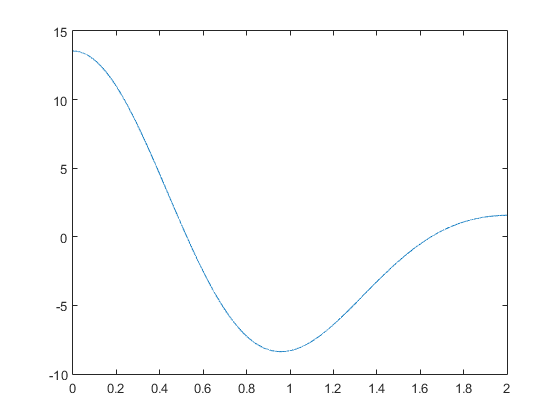
\includegraphics[width=.75\linewidth]{ch6q8c2}
					\end{center}
					\item Using the same code from part B adapted for Simpson's rule, we have that we need $48$ sub intervals for an error less than $10^{-6}$. At $n=48$ we have an error of $1.3824814e-08$
					\begin{lstlisting}
function [error] = ch6q8d(n)
% Solves for h using Simpson's rule
a = 0;
b = 2;
x = linspace(a,b,n+1);
h = x(3)-x(2);

trueError = 0.995322265;
c = ones(1,n+1);

for i=2:n
    if mod(i,2)==0 
        c(i) = 4;
    else
        c(i) = 2;
    end
end

IT = f(x);
IT = c.*IT;
IT = IT*h/3;

error = abs(trueError - sum(IT));

end

function y=f(x)
    y = 2/sqrt(pi).*exp(-x.*x);
end
					\end{lstlisting}
				\end{enumerate}
				
			\item[6.15]
				\begin{enumerate} [label={\alph*)}]
					\item Since we're given that $v(0) = 0$, and for any interval from $0$ to $t$ we get:
					\begin{align*}
					\int_{0}^{t} a(r)dr = v(t) - v(0) = v(t)
					\end{align*}
					and we know the trapezoidal rule gives us
					\begin{align*}
					\int_{0}^{t} a(r)dr = h\Big(\frac{1}{2}a_0 + \frac{1}{2}a_{t}\Big)
					\end{align*}
					we can combine the results to give us the following for the subinterval $t_i\leq t \leq t_{i+1}$
					\begin{align*}
					\int_{i}^{i+1} a(r)dr &= v(i+1) - v(i)\\
					\int_{i}^{i+1} a(r)dr &= h\Big(\frac{1}{2}a_i + \frac{1}{2}a_{i+1}\Big) \\
					v(i+1) - v(i) &= h\Big(\frac{1}{2}a_i + \frac{1}{2}a_{i+1}\Big)\\
					v(i+1) &= v(i) + \frac{1}{2}h\Big(a_i + a_{i+1}\Big)
					\end{align*}
					The same logic applies to solving for $y_{i+1}$ since we know $y(0) = 0$, and for any interval from $0$ to $t$ we get:
					\begin{align*}
					\int_{0}^{t} v(r)dr &= y(t) - y(0) = y(t)
					\end{align*}
					On the interval from $t_i\leq t \leq t_{i+1}$ we get:
					\begin{align*}
					y(i+1) - y(i) &= h\Big(\frac{1}{2}v_i + \frac{1}{2}v_{i+1}\Big)\\
					y(i+1) &= y(i) + \frac{1}{2}h\Big(v_i + v_{i+1}\Big)
					\end{align*}
					\item Plotting $y(t)$ for $n=10$, $20$, and $40$ yields the following:
					\begin{center}
						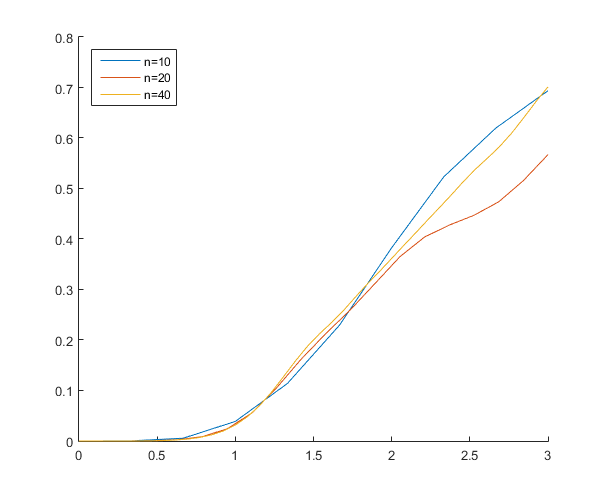
\includegraphics[width=.75\linewidth]{ch6q15b}
					\end{center}	
					\item For each value of $n$, the computed value of $y(t)$ was:
					$$\begin{array}{c|c|c}
						n & computed & difference \\ \hline
						10 & 0.69359564141 & 3.3727e-02\\
						20 & 0.56714220363 & 1.6018e-01\\
						40 & 0.70120254590 & 2.6120e-02				
					\end{array}$$
					In order to for our error to be less than 10e-8 we solve for n using the trapezoidal error. We also use Matlab to calculate $\vert \vert_\infty \leq 10^{-8}$ as :
					\begin{align*}
						\vert f'' \vert \vert_\infty \approx 1.147687e+04
					\end{align*}
					Which allows us to solve for $n$ as follows:
					\begin{align*}
						\frac{3}{12}h*2\vert \vert f'' \vert \vert_\infty &\leq 10^-8 \\
						h &\leq \sqrt{\frac{10^{-8}}{11477}*4} \quad where \quad h=\frac{3}{n} \\
						n &\geq \frac{3}{\sqrt{\frac{10^{-8}}{11477}*4}} \\
						n &\geq 160,696
					\end{align*}
				\end{enumerate}
			
			\item[6.18]
				\begin{enumerate} [label={\alph*)}]
					\item If we look first at $I_M$ we see that the function is evaluated at the midpoints between our known function values. Since Simpson's rule does not use midpoints, we need a way to convert this, and we find that by doubling the step size, our midpoint rule gives us every other function value (e.g. midpoint between $f_1$ and $f_3$, $f_3$ and $f_5$, etc.):
					\begin{align*}
						I_M(n) &= h\Big(f_{1+\frac{1}{2}} + f_{2+\frac{1}{2}}+\dots+f_{n+\frac{1}{2}}\Big) \\
						I_M(n/2) &= 2h\Big(f_2 + f_4+\dots\Big)
					\end{align*}
					
					Combining this result with the trapezoidal rule we show fairly easily that in the proportions outlined in the question, we arrive back at Simpson's rule:
					
					\begin{align*}
						I_S(n) &= \frac{2}{3}I_T(n) + \frac{1}{3}I_M\Big(\frac{n}{2}\Big) \\
						I_S(n) &= \frac{2}{3}h\Big(\frac{1}{2}f_{1} + f_{2}+\dots+\frac{1}{2}f_{n+1}\Big) + \frac{1}{3}2h\Big(f_2 + f_4+\dots\Big) \\
						I_S(n) &= \frac{h}{3}\Big(f_{1} + 2f_{2}+2f_3+\dots+f_{n+1}\Big) + \frac{h}{3}\Big(2f_2 + 2f_4+\dots\Big) \\
						I_S(n) &= \frac{h}{3}\Big(f_{1} + 4f_{2}+2f_3+\dots+f_{n+1}\Big)
					\end{align*}
					\item When we look at $I_T\Big(\frac{n}{2}\Big)$ we see a similar trend occur as in part a, where since our number of subdivisions is halved over the same interval, our step subsequently doubles, yielding:
					\begin{align*}
						I_T\Big(\frac{n}{2}\Big) &= 2h\Big(\frac{1}{2}f_1 + f_3 + f_5 + \dots+\frac{1}{2}f_{n+1}\Big) \\
						I_T\Big(\frac{n}{2}\Big) &= h\Big(f_1 + 2f_3 + 2f_5 + \dots+f_{n+1}\Big) \\
					\end{align*}
					If we plug this back into the equation given in the question, we see that again for these proportions, again, we get back Simpson's rule:
					\begin{align*}
						I_S(n) &= \frac{4}{3}I_T(n) - \frac{1}{3}I_T\Big(\frac{n}{2}\Big) \\
						I_S(n) &= \frac{4}{3}h\Big(\frac{1}{2}f_{1} + f_{2}+\dots+\frac{1}{2}f_{n+1}\Big) - \frac{1}{3}h\Big(f_1 + 2f_3 + 2f_5 + \dots+f_{n+1}\Big) \\
						I_S(n) &= \frac{h}{3}\Big(2f_{1} + 4f_{2}+4f_3+\dots+2f_{n+1}\Big) - \frac{h}{3}\Big(f_1 + 2f_3 + 2f_5 + \dots+f_{n+1}\Big) \\
						I_S(n) &= \frac{h}{3}\Big(f_{1} + 4f_{2}+2f_3+\dots+f_{n+1}\Big)
					\end{align*}
				\end{enumerate}
				
			\item[6.19]
				\begin{enumerate} [label={\alph*)}]
					\item We know from the trapezoidal rule that we have
					$$I_T = h\Big(\frac{1}{2}f_{i-1} + f_i + \frac{1}{2}f_{i+1}\Big)$$ However, since we don't know the value of $f$ at $x_i$ we need to find a way to exclude it during out calculation. We do this by increasing the step size $h$ so we evaluate only at the end points $x_{i-1}$ and $x_{i+1}$:
					\begin{align*}
						I_T &= 2h\Big(\frac{1}{2}f_{i-1} + \frac{1}{2}f_{i+1}\Big) \\
						&= h\Big(f_{i-1} + f_{i+1}\Big)
					\end{align*}					 
					\item If we use linear interpolation to find a value for $f_i$ we see from the plot below that $f_i$ takes the value:
					\begin{center}
						$f_i = \frac{f_{i+1}+f_{i-1}}{2}$ \\
						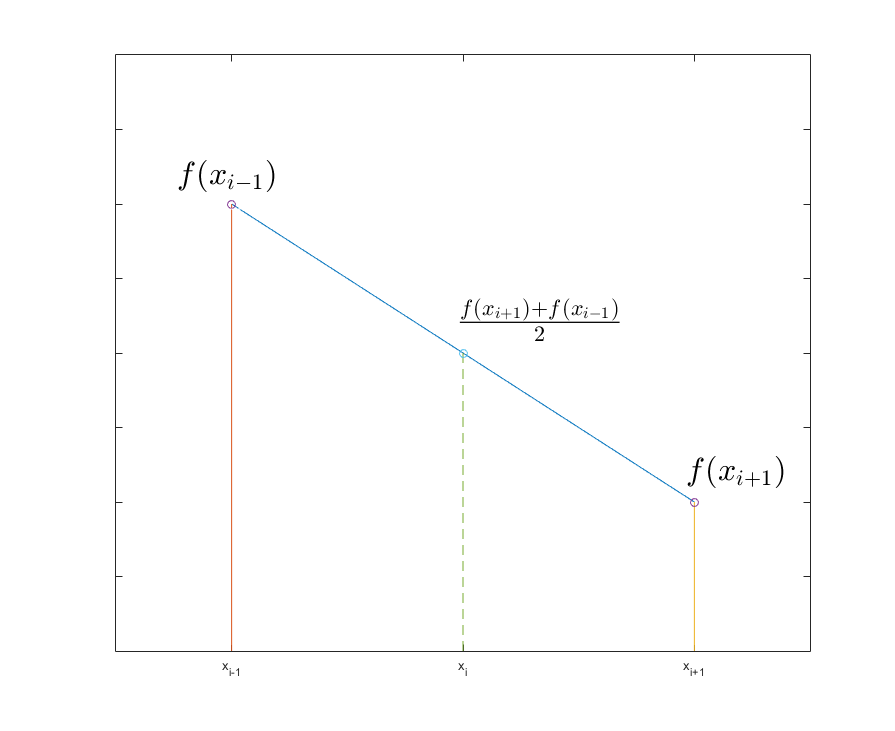
\includegraphics[width=1\linewidth]{ch6q19b}
					\end{center}
					If we take this value of $f_i$ and substitute it into Simpson's rule we get, by simplifying, the following:
					\begin{align*}
						I_S &= \frac{h}{3}\Big(f_{i-1} + 4f_i + f_{i+1}\Big) \\
						&= \frac{h}{3}\Big(f_{i-1} + 4\big(\frac{f_{i+1}+f_{i-1}}{2}\big) + f_{i+1}\Big) \\
						&= \frac{h}{3}\Big(f_{i-1} + 2\big(f_{i+1}+f_{i-1}\big) + f_{i+1}\Big) \\
						&= \frac{h}{3}\Big(3f_{i-1} + 3f_{i+1}\Big) \\
						&= h\Big(f_{i-1} + f_{i+1}\Big)
					\end{align*}
					We see this is the same result we reached in part (a)
					\item If we assume there are constants $A$ and $B$, we can plug these into Simpson's rule to solve for the weights that maximize precision as follows:
					\begin{align*}
						I_S &= \frac{h}{3}\Big(f_{i-1} + 4f_i + f_{i+1}\Big) \\
						&= \frac{h}{3}\Big(f_{i-1} + 4\big(Af_{i-1} + Bf_{i+1}\big) + f_{i+1}\Big) \\
						&= \frac{h}{3}\Big((4A+1)f_{i-1} + (4B+1)f_{i+1}\Big) \\
						&= \frac{(4A+1)h}{3}f_{i-1} + \frac{(4B+1)h}{3}f_{i+1}
					\end{align*}
					where $$w_1 = \frac{(4A+1)h}{3}, \quad w_2 = \frac{(4B+1)h}{3}$$ Here we also note that $w_1$ and $w_2$ appear to be symmetric, differing only by their respective values of $A$ and $B$, which are likely to be symmetric around some point.
					
				\end{enumerate}
				
			\item[6.20]
				\begin{enumerate} [label={\alph*)}]
					\item It's given that the error involved with Simpson's rule takes the form
					$$I_S(n) + \alpha h^4 + \beta h^6 + \gamma h^8 + \dots$$
					and so substituting in the known error for $I_S(n)$ and $I_S(n/2)$ yields the following:
					\begin{align*}
						I_R &= \frac{1}{15}\Big[ 16I_S(2n)-I_S\Big] \\
						I_R &= \frac{1}{15}\Big[ 16(\alpha\frac{h}{2}^4 + \beta\frac{h}{2}^6 + \gamma\frac{h}{2}^8+\dots) - (\alpha h^4 + \beta h^6 + \gamma h^8+\dots)\Big] \\
						I_R &= \frac{1}{15}\Big[ \alpha\frac{16h^4}{16} + \beta\frac{16h^6}{64} + \gamma\frac{h}{2}^8+\dots) - (\alpha h^4 + \beta h^6 + \gamma h^8+\dots)\Big] \\
						I_R &= \frac{1}{15}\Big[ \alpha h^4 + \beta\frac{h^6}{4} + \gamma\frac{h}{2}^8+\dots) - (\alpha h^4 + \beta h^6 + \gamma h^8+\dots)\Big] \\ 
						I_R &= \frac{1}{15}\Big[ \beta\frac{h^6}{4} + \gamma\frac{h}{2}^8+\dots) - (\beta h^6 + \gamma h^8+\dots)\Big]
					\end{align*}
					We assume here that since the number of sub intervals is doubled, the step size is necessarily halved. Also, we see the $\alpha$ error term is eliminated, leaving the dominant term here as $h^6$ meaning $I_R = O(h^6)$
					\item Here we have that the error associated with $f(x)$ is equal to $$\int_a^b f(x)dx = I(n) + \alpha h^2 + \beta h^3 + \gamma h^4 + \dots$$
					By adjusting the step size within the same interval to account for increased numbers of $n$ sub intervals we solve for $I_R$ as
					\begin{align*}
						I_R &= \frac{1}{21}\Big[32I(4n) - 12I(2n) + I(n)\Big] \\
						&= \frac{1}{21}\Big[32\Big(\alpha \big( \frac{h}{4}\big)^2 + \beta\big(\frac{h}{4}\big)^3 + \gamma\big(\frac{h}{4}\big)^4\Big) - 12\Big(\alpha\big(\frac{h}{2}\big)^2 + \beta\big(\frac{h}{2}\big)^3 + \gamma\big(\frac{h}{2}\big)^4\Big) + \Big(\alpha h^2 + \beta h^3 + \gamma h^4\Big)\Big] \\
						&= \frac{1}{21}\Big[32\Big(\alpha \frac{h^2}{16} + \beta\frac{h^3}{64} + \gamma\frac{h^4}{256}\Big) - 12\Big(\alpha\frac{h^2}{4} + \beta\frac{h^3}{8} + \gamma\frac{h^4}{16}\Big) + \Big(\alpha h^2 + \beta h^3 + \gamma h^4\Big)\Big] \\
						&= \frac{1}{21}\Big[\Big(2\alpha h^2 + \frac{1}{2}\beta h^3 + \frac{1}{8}\gamma h^4\Big) - \Big(3\alpha h^2 + \frac{3}{2}\beta h^3 + \frac{3}{4}\gamma h^4 \Big) + \Big(\alpha h^2 + \beta h^3 + \gamma h^4\Big)\Big]
					\end{align*}
					Combining like terms we reduce this to
					\begin{align*}
						I_R &= \frac{1}{21}\Big[\Big(2\alpha h^2 - 3\alpha h^2 + \alpha h^2 \Big) + \Big( \frac{1}{2}\beta h^3 - \frac{3}{2}\beta h^3 + \beta h^3 \Big) + \Big( \frac{1}{8}\gamma h^4 - \frac{3}{4}\gamma h^4 + \gamma h^4 \Big) \Big] \\ 
						&= \frac{1}{21}\Big[\Big( \frac{3}{8} \gamma h^4\Big)\Big]
					\end{align*}
					From this we see that the $\alpha$ and $\beta$ terms cancel out and we are left with an error that is $O(h^4)$
					
					\item Here we have that the error associated with $f(x)$ is equal to $$\int_a^b f(x)dx = I(n) + \alpha h^2 + \beta h^3 + \gamma h^4 + \dots$$
					Again, by adjusting the step size within the same interval to account for increased numbers of $n$ sub intervals we solve for $I_R$ as
					\begin{align*}
						I_R &= \frac{1}{12}\Big[27I(3n) - 16I(2n) + I(n)\Big] \\
						&= \frac{1}{12}\Big[27\Big(\alpha \big( \frac{h}{3}\big)^2 + \beta\big(\frac{h}{3}\big)^3 + \gamma\big(\frac{h}{3}\big)^4\Big) - 16\Big(\alpha\big(\frac{h}{2}\big)^2 + \beta\big(\frac{h}{2}\big)^3 + \gamma\big(\frac{h}{2}\big)^4\Big) + \Big(\alpha h^2 + \beta h^3 + \gamma h^4\Big)\Big] \\
						&= \frac{1}{12}\Big[27\Big(\alpha \frac{h^2}{9} + \beta\frac{h^3}{27} + \gamma\frac{h^4}{81}\Big) - 16\Big(\alpha\frac{h^2}{4} + \beta\frac{h^3}{8} + \gamma\frac{h^4}{16}\Big) + \Big(\alpha h^2 + \beta h^3 + \gamma h^4\Big)\Big] \\
						&= \frac{1}{12}\Big[\Big(3\alpha h^2 + \beta h^3 + \frac{1}{3}\gamma h^4\Big) - \Big(4\alpha h^2 + 2\beta h^3 + \gamma h^4 \Big) + \Big(\alpha h^2 + \beta h^3 + \gamma h^4\Big)\Big]
					\end{align*}
					Combining like terms we reduce this to
					\begin{align*}
						I_R &= \frac{1}{12}\Big[\Big(3\alpha h^2 - 4\alpha h^2 + \alpha h^2 \Big) + \Big(\beta h^3 - 2\beta h^3 + \beta h^3 \Big) + \Big( \frac{1}{3}\gamma h^4 - \gamma h^4 + \gamma h^4 \Big) \Big] \\ 
						&= \frac{1}{12}\Big[\Big( \frac{1}{3} \gamma h^4\Big)\Big]
					\end{align*}
					From this we see that the $\alpha$ and $\beta$ terms cancel out and we are left with an error that is $O(h^4)$
					
				\end{enumerate}
				
			\item[6.21]
				\begin{enumerate} [label={\alph*)}]
					\item Since we're solving for three unknowns, we need at least 3 equations. These are given in the book in Table 6.5 as:
					$$\begin{array}{|c|c|c|}
						k & f(x) & \displaystyle\int_{x_i}^{x_{i+1}} f(x)dx) \\ \hline
						0 & 1 & h \\
						1 & x & h\Big(x_i + \frac{1}{2}h\Big) \\
						2 & x^2 & h\Big(x_i^2 + hx_i + \frac{1}{3}h^2 \Big)
					\end{array}$$
					
					First taking $k=0$ we solve for $w_1$:
					\begin{align*}
						h &= w_1 + w_2 \\
						w_1 &= h - w_2
					\end{align*}
					
					Using our second formula we solve for $w_2$ remembering that in the problem, $z$ is given as $x_i + \alpha h$ where we are to solve for $\alpha$:
					\begin{align*}
						h\Big(x_i + \frac{1}{2}h\Big) &= w_1x_i + w_2z \\
						&= (h-w_2)x_i + w_2x \\
						hx_i + \frac{1}{2}h^2 &= hx_i-w_2x_i+w2_z \\
						\frac{1}{2}h^2 &= -w_2x_i+w_2z \\
						\frac{h^2}{2} &= w_2(z - x_i) \\
						\frac{h^2}{2} &= w_2(x_i + \alpha h - x_i) \\
						\frac{h^2}{2} &= w_2(\alpha h) \\
						w_2 &= \frac{h}{2\alpha}
					\end{align*}
					
					Using our third formula and having equations in place for $w_1$ and $w_2$ we can solve for $\alpha$ as follows:
					\begin{align*}
					h\Big(x_i^2 + hx_i + \frac{1}{3}h^2 \Big) &= w_1x_i^2 + w_2z^2 \\
					&= (h-w_2)x_i^2 + w_2z^2 \\
					&= hx_i^2-w_2x_i^2 + w_2(x_i+\alpha h)^2 \\
					&= hx_i^2-w_2x_i^2 + w_2(x_i^2 + 2x_i \alpha h + \alpha^2 h^2) \\
					&= hx_i^2 + w_2(2x_i \alpha h + \alpha^2 h^2) \\
					&= hx_i^2 + \frac{h}{2\alpha}(2x_i \alpha h + \alpha^2 h^2) \\
					hx_i^2 + h^2x_i+\frac{h^3}{3} &= hx_i^2 + h^2x_i+\frac{h^3\alpha}{2} \\
					\frac{h^3}{3} &= \frac{h^3\alpha}{2} \\
					\alpha &= \frac{2}{3}
					\end{align*}
					\item From Theorem 6.5 we have $$E_G = Kh^{2\ell + 1}f^{(2\ell)}\big(\eta\big)$$ where $K$ is given to be $$\frac{(\ell!)^4}{(2\ell +1)[(2\ell)!]^3}$$ Since we have 2-point Gaussian quadrature but one of the points is fixed, we are left with $\ell = 1$. Plugging this into our equation for $K$ we see:
					\begin{align*}
						K &= \frac{(1!)^4}{(2+1)[(2)!]^3} \\
						  &= \frac{1}{(3)(2)^3} \\
						  &= \frac{1}{24}
					\end{align*}
				\end{enumerate}
		\end{itemize}	
	
\end{document}